% Подписи колонтитула
\newcommand{\colontitulAutors}{edombek, astronom\_v\_cube et al.}
\newcommand{\colontitulYear}{2022}
\newcommand{\colontitulEducationalSubject}{Прикладная электродинамика}
\newcommand{\colontitulTeacher}{Гиндельбург~В.~Б.}

%Настройки шаблона
\documentclass[10pt,landscape,a4paper]{article}
\usepackage[utf8]{inputenc}
\usepackage[english, russian]{babel}
\usepackage[T1,T2A]{fontenc}  
\usepackage{upgreek} % прямые греческие ради русской традиции
\usepackage{tikz}
\usetikzlibrary{shapes,positioning,arrows,fit,calc,graphs,graphs.standard}
%\usepackage[nosf]{kpfonts}
%\usepackage[t1]{sourcesanspro}
\usepackage{multicol}
\usepackage{wrapfig}
\usepackage[top=6mm,bottom=8mm,left=4mm,right=4mm]{geometry}
\usepackage[framemethod=tikz]{mdframed}
\usepackage{microtype}
\usepackage{pdfpages}
\usepackage{amsthm,amsmath,amscd}   % Математические дополнения от AMS
\usepackage{amsfonts,amssymb}       % Математические дополнения от AMS
\usepackage{mathtools}              % Добавляет окружение multlined
\usepackage{xfrac}                  % Красивые дроби
\usepackage{physics}

\usepackage{fancyhdr} % колонтитулы

%некоторые математические команды
\newcommand{\Div}{\operatorname{div}}
\newcommand{\Grad}{\operatorname{grad}}

\let\bar\overline

\definecolor{myblue}{cmyk}{1,.72,0,.38}

\def\firstcircle{(0,0) circle (1.5cm)}
\def\secondcircle{(0:2cm) circle (1.5cm)}

\colorlet{circle edge}{myblue}
\colorlet{circle area}{myblue!5}

\tikzset{filled/.style={fill=circle area, draw=circle edge, thick},
	outline/.style={draw=circle edge, thick}}

\pgfdeclarelayer{background}
\pgfsetlayers{background,main}

%\everymath\expandafter{\the\everymath \color{myblue}}
\everydisplay\expandafter{\the\everydisplay \color{myblue}}

\renewcommand{\baselinestretch}{.8}
\pagestyle{empty}

\global\mdfdefinestyle{header}{%
	linecolor=gray,linewidth=1pt,%
	leftmargin=0mm,rightmargin=0mm,skipbelow=0mm,skipabove=0mm,
}

\makeatletter % Author: ttps://tex.stackexchange.com/questions/218587/how-to-set-one-header-for-each-page-using-multicols
\renewcommand{\section}{\@startsection{section}{1}{0mm}%
	{.2ex}%
	{.2ex}%x
	{\color{myblue}\sffamily\small\bfseries}}
\renewcommand{\subsection}{\@startsection{subsection}{1}{0mm}%
	{.2ex}%
	{.2ex}%x
	{\sffamily\bfseries}}

\makeatother
\setlength{\parindent}{0pt}

%колонтитулы
\pagestyle{fancy}
\fancyhf{}
\setlength{\headheight}{40pt}
\setlength{\headsep}{4pt}
\renewcommand{\headrulewidth}{1pt}
\fancyhead[L]{\textcopyright~\colontitulAutors}
\fancyhead[C]{Программа минимум по курсу <<\colontitulEducationalSubject>> \colontitulYear г}
\fancyhead[R]{Преподаватель:~\colontitulTeacher}

\renewcommand{\frac}{\dfrac} % большие дроби
\renewcommand{\k}{\varkappa}
\newcommand{\eps}{\varepsilon}
\newcommand{\w}{\omega}
\newcommand\deriv[3]{\ensuremath{\frac{\partial^{#1} {#2}}{\partial {#3}^{#1}}}}

\begin{document}
	\small
	\begin{multicols*}{2}
		\section{Запись функции, определяющей зависимость полей и векторных потенциалов гармонической плоской волны в линии передачи от времени $t$ и продольной координаты $z$. Понятия частоты, временного периода, продольного волнового числа, длины волны, фазовой и групповой скорости.}
		
		$\{\vec{E},\vec{H}\}=\{\vec{E_0},\vec{H_0}\}e^{i(\w t-hz)}, ~\vec{A}^{e,m}=\vec{z_0}\psi^{e,m}(r_{\perp})e^{-ihz}$ \\
		$\psi$~-~произвольная скалярная функция (амплитуда векторного потенциала), $(\w t-hz)$~-~фаза \\
		$k=\frac wc\sqrt{\mu\eps}$~-~волновое число в среде, $ h $~-~ продольное волновое число. \\
		$T=\frac {2\pi}\w, \lambda_\text{в}=\frac {2\pi}h, V_\text{ф}=\frac{\w}{h}, V_\text{гр}=\dv{\w}{h}$. Для волновода без заполнения $V_\text{ф}V_\text{гр}=c^2$. $V_\text{гр}\le c$.
		
		\section{Волновое уравнение для векторного потенциала в отсутствие источников при произвольной и гармонической зависимости от времени. Дифференциальное уравнение для скалярных поперечных волновых функций $\psi^{(e),(m)}(r_\perp)$, определяющих зависимость полей в линии передачи от поперечных координат. Понятие поперечного волнового числа. }
		
		$\Delta \vec{A}+k^2\vec{A}=0, \quad \Delta=\frac{\partial^2}{\partial z^2}+\Delta_\perp,\quad \Delta_\perp=\frac{\partial^2}{\partial x^2}+\frac{\partial^2}{\partial y^2},\quad \frac{\partial^2}{\partial z^2}=-h^2$. \\
		При гармонической зависимости от $t$: $\Delta \vec{A_\perp}+(k^2-h^2)\vec{A}=0$.\\
		Решение: $\vec{A}^{e,m}=\vec{z_0}\psi^{e,m}(r_\perp)e^{-ihz}$ (в отсутствии сторонних источников); \\
		TE($ E_z=0 $): $ \Delta_\perp\psi^m+\varkappa^2\psi^m=0 $; \\
		TM($ H_z=0 $): $ \Delta_\perp\psi^e+\varkappa^2\psi^e=0 $; \\
		TEM($ E_z=0 $): $ \Delta_\perp\psi=0 $.\\
		$\varkappa^2=k^2-h^2$~-~поперечное волновое число. \\
		$\varkappa_n=\sqrt{\frac{\w^2}{c^2}\mu\eps-h_n^2}, \quad n=0,1,2,...$~-~номер моды.
		
		\section{Понятие о ТЕ, ТМ и ТЕМ волнах. Импедансная связь поперечных компонент полей. Определение поперечного волнового импеданса. }
		
		$\{\vec{H},\vec{E}\}=\vec{z_0}\{{H_z},{E_z}\}+\{\vec{H_\perp},\vec{E_\perp}\}$ \\
		\begin{tabular}{l l l}
			TM~($H_z=0$) & TE~($E_z=0$) & TEM~($E_z=H_z=0$) \\
			$\begin{rcases}
				E_z=\frac{\varkappa^2}{ik_0\eps\mu}\psi^e \\
				\vec{E_\perp} = \frac{-h}{k_0\eps\mu}\nabla_\perp\psi^e \\
				\vec{H_\perp}=\frac1{\mu}[\nabla_\perp\psi^e,\vec{z_0}]
			\end{rcases} e^{i(\w t-hz)}$ & 
			$\begin{rcases}
				H_z=\frac{\varkappa^2}{ik_0\eps\mu}\psi^m \\
				\vec{H_\perp} = \frac{-h}{k_0\eps\mu}\nabla_\perp\psi^m \\
				\vec{E_\perp}=\frac{-1}{\eps}[\nabla_\perp\psi^m,\vec{z_0}]
			\end{rcases} e^{i(\w t-hz)}$ & 
			$\begin{rcases}
				\vec{E_\perp} =-\frac1{\sqrt{\eps\mu}}\nabla_\perp\psi \\
				\vec{H_\perp}=\frac1{\mu}[\nabla_\perp\psi,\vec{z_0}]
			\end{rcases} e^{i(\w t-hz)}$ \\
		\end{tabular}
		$\vec{E}_\perp=\zeta_\perp[\vec{H_\perp},\vec{z_0}]$~-~импедансная связь \\
		Поперечный импеданс \textbf{в бегущей плоской волне} ($\zeta_\perp$): \\
		\begin{tabular}{l l l}
			TE & TM & TEM \\
			$\sqrt{\frac{\mu}{\eps}}\frac kh$ & $\sqrt{\frac{\mu}{\eps}}\frac hk$ & $\sqrt{\frac{\mu}{\eps}}$ \\
		\end{tabular}
		
		\section{Граничные условия для полей и поперечных волновых функций $\psi^{(e)}$ и $\psi^{(m)}$ в линиях передачи с идеально проводящими границами. Математическая формулировка задачи отыскания собственных волн различных типов в идеальной линии.}
		
		$E_\tau=0,~H_n=0$ - Г.~У. \\
		\begin{tabular}{l l l}
			TE: & TM: & TEM: \\
			$\begin{cases}
				\Delta_\perp\psi^m+\varkappa^2\psi^m=0 \\
				\pdv{\psi^m}{n}|_{L}=0 \text{~-~условие Неймана}\\
			\end{cases}$  &
			$\begin{cases}
				\Delta_\perp\psi^e+\varkappa^2\psi^e=0 \\
				\psi^e|_{L}=0 \text{~-~условие Дирихле}\\
			\end{cases}$  &
			$\begin{cases}
				\Delta_\perp\psi=0 \\
				\psi=const_i|_{L_i}\\
			\end{cases}$ \\
		\end{tabular}
		
		\section{Дисперсионное уравнение для волн в идеальных линиях. Понятие критической частоты и критической длины волны. Графики зависимости полей от продольной координаты в различные моменты времени при частотах, больших или меньших критической. Зависимости длины волны, фазовой и групповой скорости в линии передачи от частоты.}
		
		$h_n = \pm \sqrt{k^2 - \varkappa^2} = \pm \sqrt{\dfrac{\omega^2 \varepsilon \mu}{c^2} - \varkappa_n^2}$, \quad $n = 1,~2,~3...$ - номер моды\\
		В ИЛП есть бесконечные наборы $ТЕ$ и $ТМ$ волн, называемые модой. Любой моде соответствует своё дисперсионное соотношение. При этом $\varkappa_n$ не зависит от $\omega,~\varepsilon,~\mu$, а определяется геометрией ЛП.\\
		Существует критическая частота, при которой осуществляется переход от распространения волны к нераспространению.\\
		$\omega_\text{кр n} = \dfrac{\varkappa_n c}{\sqrt{\varepsilon \mu}}$; \quad $\lambda_\text{кр n} = \dfrac{2\pi \sqrt{\varepsilon \mu}}{\varkappa_n}$.\\
		\begin{tabular}{l l}
			{Распространение} & {Нераспространение} \\
			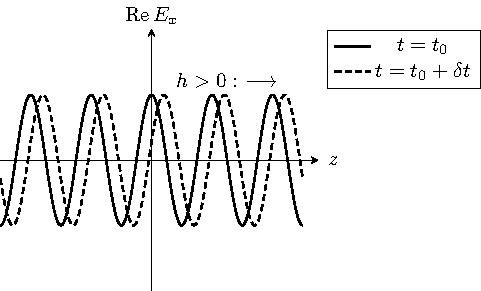
\includegraphics[width=0.25\linewidth]{aed_imgs/lect3_ris1} &
			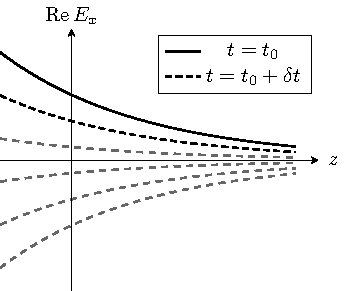
\includegraphics[width=0.25\linewidth]{aed_imgs/lect3_ris2} \\
		\end{tabular} \\
		$\lambda_\text{в}=2\pi/h=\frac{\lambda_0}{\sqrt{1-\frac{\w_\text{кр}^2}{\w^2}}};\quad V_\text{гр}=c \sqrt{1-\frac{\w_\text{кр}^2}{\w^2}};\quad V_\text{ф}=\frac{c}{\sqrt{1-\frac{\w_\text{кр}^2}{\w^2}}}$.
		
		\section{В каких линиях могут существовать главные (ТЕМ) волны? Поля ТЕМ волны в коаксиальной линии (форма силовых линий и зависимость от координат).}
		
		TEM-волна~--~волна, где присутствуют только поперечные компоненты полей ($E_z = H_z = 0) \Rightarrow h = k$,~ $\varkappa = 0$. Предположим, что в волноводе распространяется волна, у которой векторы $\vec{E}$ и $\vec{H}$ лежат в поперечной плоскости. Силовые линии вектора $\vec{H}$, являясь замкнутыми, должны охватывать линии тока. Но токи проводимости отсутствуют, поскольку внутри волновода проводников нет. Значит, током может быть только продольный ток смещения. Поэтому должна иметься продольная составляющая вектора. Следовательно, ТЕМ-волна (волна без продольной составляющей вектора) в волноводе не может распространяться. Из этих рассуждений ясно, что для существования ТЕМ-волны в замкнутой направляющей системе необходимо, чтобы последняя состояла \textbf{не менее чем из двух изолированных друг от друга проводников}, по которым может протекать ток проводимости (коаксиальная линия, полосковая и пр.)\\
		$E_r = \dfrac{const}{r} = \zeta_\perp H_\theta$ - поле обратно пропорционально $r$\\
		\begin{tabular}{l}
			{Поле в коаксиальном кабеле} \\
			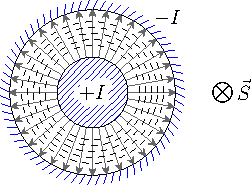
\includegraphics[width=0.25\linewidth]{aed_imgs/lect4_ris6} \\
		\end{tabular}
		
		\section{Спектр поперечных волновых чисел прямоугольного волновода. Низшая мода (поперечное волновое число, графики поля, картина силовых линий). Низшая мода круглого волновода (поперечное волновое число, картина силовых линий).}
		
		$\k_{mn}^2=\qty(\frac{m\pi}{a})^2+\qty(\frac{n\pi}{b})^2, \{m,n\} = (0),1,2,3...$ \\
		Низшая мода – мода, которой соответствует наименьшее поперечное волновое число ($\k=\k_\text{min}$), соответственно, наименьшая частота ($\omega =\omega_\text{min}$) \\
		\begin{tabular}{r *{2}{c}}
			{} & {Прямоугольный} & {Круглый} \\
			{$\k_{mn}$} &
			{$\sqrt{\qty(\frac{m\pi}{a})^2+\qty(\frac{n\pi}{b})^2}$} &
			{$\begin{cases}
					\frac{\mu_{mn}}{a}, \quad \text{TE} \\
					\frac{\nu_{mn}}{a}, \quad \text{TM}\\
				\end{cases}$} \\
			{Низшая мода} & {$\text{TE}_{10}$} & {$\text{TE}_{11}$} \\
			{$\k_\text{min}$} & {$\frac \pi a$} & {$\frac {\mu_{11}}{a}=\frac {1.84}{a}$} \\
			{Распределение поля} &
			{\begin{tabular}{c}
					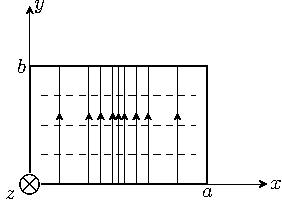
\includegraphics[width=0.25\linewidth]{aed_imgs/lect4_ris8} \\
					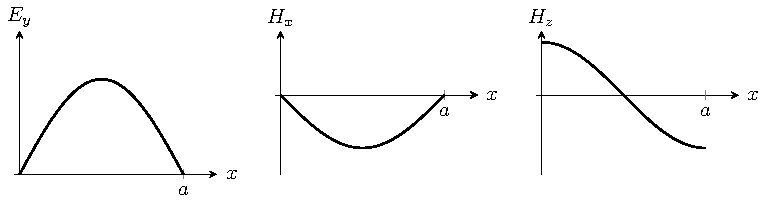
\includegraphics[width=0.25\linewidth]{aed_imgs/lect4_ris9} \\
					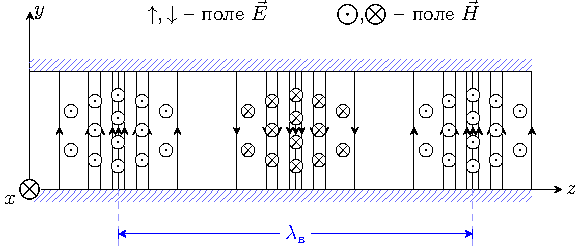
\includegraphics[width=0.25\linewidth]{aed_imgs/lect4_ris10} \\
			\end{tabular}} &
			{\begin{tabular}{c}
					{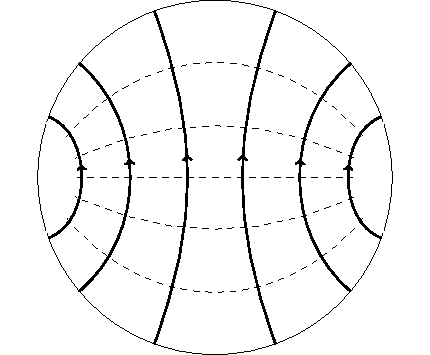
\includegraphics[width=0.25\linewidth]{aed_imgs/lect5_cylindric_TE11}} \\
					$m$ - порядок функции Бесселя\\
					$n$ - номер нуля производной\\ или нуля функции Бесселя\\
					ТЕ: $\mu$ - ноль производной \\ функции Бесселя\\
					ТМ: $\nu$ - ноль производной \\ функции Бесселя
			\end{tabular}}\\
			{} & \multicolumn{2}{c}{($\vec{H}$ пунктиром)} \\
		\end{tabular}
		
		\section{Причины затухания волн в линиях передачи. Описание затухания, обусловленного потерями энергии в заполняющей среде. Графики зависимости поля в линии передачи с потерями от продольной координаты в различные моменты времени.}
		
		Потери могут быть вызваны потерями энергии в заполняющей среде и на стенках (конечная проводимость). \\
		$\eps=\eps'+i\eps'', \mu=\mu'+i\mu'' \Rightarrow h=h'+ih''$  - комплексные части дают потери в заполняющей среде. \\
		$E_x\sim e^{i(\w t-hz)}=e^{-h''z}e^{i(\w t-h'z)}$,\quad $\Re(E_x) \sim cos~e^{-h'' z}$, \quad $\abs{h''}$~-~декремент затухания. \\
		$h' = \sqrt{\frac{\omega^2}{c^2} \eps' - \varkappa^2}, \quad h'' = \frac{\eps'' k_{0}^2}{2 h'}\quad (\mu=1)$. \\
		$Q = \w \dfrac{\bar{W^T}}{P_{\text{пот}}} = 2\pi \dfrac{\bar{W^T}}{T P_{\text{пот}}} = \dfrac{\w'}{2\w''}$ - добротность\\
		\begin{tabular}{l}
			{Зависимость поля в линии передачи с потерями} \\
			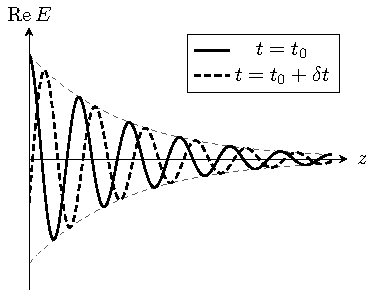
\includegraphics[width=0.25\linewidth]{aed_imgs/ask8_1} \\
		\end{tabular}
		
		\section{Описание главных волн в линиях передачи в терминах тока и напряжения: определения величин тока и напряжения, погонной емкости и индуктивности, определения волнового сопротивления, импеданса нагрузки, импеданса в любом сечении линии с произвольной нагрузкой на конце.}
		
		$V=\int\limits_1^2E_ldl$ \\
		$\pdv{Q_\text{лин}}{t}=-\pdv{I}{z}$, где $Q_\text{лин}$~-~линейный заряд на единицу длинны; $I$~-~сила тока в направлении $z$ \\
		Главные волны можно описать с помощью телеграфных уравнений: \\
		$\pdv{I}{z}=-C\pdv{V}{t}$, \quad $\pdv{V}{z}=-\frac{1}{c^2}L\pdv{I}{t}$ \\
		где $C=\frac{Q_\text{лин}}{V}$~-~погонная ёмкость; $L$~-~погонная индуктивность.\\
		Из них можно получить волновое уравнение: \\
		$\deriv2{V}{z}-\frac{LC}{c^2}\deriv2{V}{t}=0$,\quad $U=\frac{c}{\sqrt{LC}}$~-~скорость распространения волны. \\
		$Z_\text{в}=\frac 1c\sqrt{\frac LC}$~-~волновое сопротивление; \quad
		$Z_\text{н}=\frac{V_\text{н}}{I_\text{н}}$~-~импеданс нагрузки; \\
		$Z(z)=\frac{V(z)}{I(z)}$~-~комплексный импеданс линии передачи; \\
		$Z(z)\neq Z_\text{в}$~-~по причине отражения.\\
		$Z(-L) = Z_\text{в} \dfrac{Z_\text{н}+iZ_\text{в}tg(kL)}{Z_\text{в}+iZ_\text{н}tg(kL)}$ - формула пересчета импедансов
		
		\section{Коэффициент отражения волны от нагрузки на конце линии. Понятие согласования линии с нагрузкой.}
		
		На нагрузке: $\Gamma=\frac {V_r}{V_i}$, где $r, i$~-~обозначают отражённую и падающую волну соответственно. \\
		$\Gamma=\frac{Z_\text{н}-Z_\text{в}}{Z_\text{н}+Z_\text{в}}$. \\
		$Z_\text{н}=0 \Rightarrow \Gamma=-1$ ~-~коротко замкнут; \\
		$Z_\text{н}=\infty \Rightarrow \Gamma=1$ ~-~разомкнут; \\
		$Z_\text{н}=Z_\text{в} \Rightarrow \Gamma=0$ ~-~\textbf{согласование} (отсутствие отражения).
		
		\section{Спектр собственных частот идеального прямоугольного резонатора. Низшая мода прямоугольного резонатора (собственная частота, структура поля).}
		
		$\omega_{mnp}^2=\dfrac{c^2}{\varepsilon\mu}\qty(\qty(\dfrac{m\pi}{a})^2+\qty(\dfrac{n\pi}{b})^2+\qty(\dfrac{p\pi}{L})^2),\quad \{m,n,p\} = (0),1,2,3,...$ \\
		Мода это собственное колебание, характеризующееся собственной частотой и своей структурой поля.\\
		В прямоугольном резонаторе: $b < a$,~$b < L$, где $L$ - продольный размер резонатора $\Rightarrow m = 1, n = 0, p = 1$ - низшая мода\\
		Низшая мода: ${\text{TEM}}_{101} \rightarrow \omega_{101}^2 = \dfrac{c^2}{\varepsilon\mu}\qty(\qty(\dfrac{\pi}{a})^2+\qty(\dfrac{\pi}{L})^2)$ \\
		\begin{tabular}{l l l}
			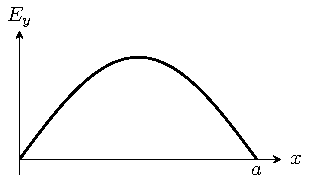
\includegraphics[width=0.25\linewidth]{aed_imgs/ask11_1} &
			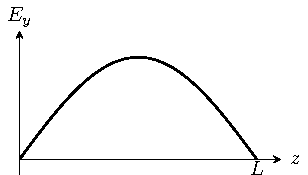
\includegraphics[width=0.25\linewidth]{aed_imgs/ask11_2} &
			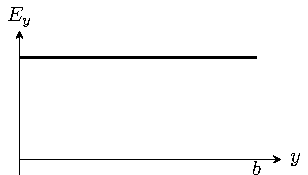
\includegraphics[width=0.25\linewidth]{aed_imgs/ask11_3} \\
		\end{tabular}
		
		\section{Причины затухания колебаний в реальных резонаторах. Описание затухания, обусловленного потерями энергии в заполняющей среде. График зависимости поля собственного колебания в реальном резонаторе от времени.}
		
		Основные причины затухания - это потери в среде и потери в стенках.\\
		$\eps=\eps'+i\eps'', \mu=\mu'+i\mu'' \Rightarrow \w_\text{рез}=\w_\text{рез}'+i\w_\text{рез}''$  - комплексные части дают потери в заполняющей среде. \\
		$\Re(E_x)\sim cos(\omega't)e^{-\w''_\text{рез}t}$,\quad $\abs{\w''_\text{рез}}$~-~декремент затухания. \\
		$\w_\text{рез} = \dfrac{\w_\text{0 рез}}{\sqrt{\varepsilon \mu}} = \dfrac{ck_\text{рез}}{\sqrt{\varepsilon \mu}}, \quad \vec{E},\vec{H} \sim e^{i\omega_\text{рез}t} = e^{i\omega_\text{рез}'t}e^{-\omega''t}$\\
		$\w_\text{рез}' = \sqrt{\dfrac{\w_\text{0 рез}^2}{c^2}(\varepsilon' \mu') - \varkappa^2}, \quad \w_\text{рез}'' = \dfrac{(\varepsilon'' \mu' + \varepsilon' \mu'')k^2_0}{2w'_\text{рез}}$ (общий случай $\eps$ и $\mu$ - комплексные)\\
		\begin{tabular}{l}
			{Зависимость поля во времени в резонаторе с потерями} \\
			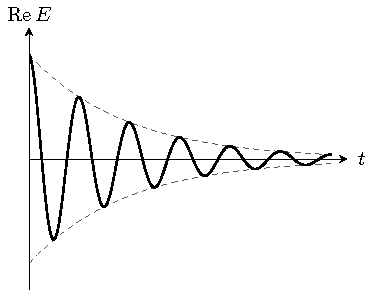
\includegraphics[width=0.25\linewidth]{aed_imgs/ask12_1} \\
		\end{tabular}
		
		\section{Представление полей, создаваемых в волноводе заданными сторонними токами, в виде суперпозиции полей собственных мод (общий вид формул возбуждения волноводов).}
		
		$\vec{E} = \sum\limits_{p = 1}^{\infty} a_p\vec{E_p}, \quad \vec{H} = \sum\limits_{p = 1}^{\infty} a_p\vec{H_p}$ \quad при распространении $\longrightarrow $\\
		$\vec{E} = \sum\limits_{p = 1}^{\infty} a_{(-p)}{\vec{E}}_{(-p)}, \quad \vec{H} = \sum\limits_{p = 1}^{\infty} a_{(-p)}\vec{H}_{(-p)}$ \quad при распространении $\longleftarrow $\\
		$\vec{E_{p}}, \vec{H_{p}}$ - собственные моды, \quad $p$ = 1, 2, 3 - индексы мод\\
		$\begin{rcases}
			a_p = \dfrac{1}{N_p} \int\limits_{V}(\vec{j}^{e}{\vec{E}}_{(-p)} - \vec{j}^{m}{\vec{H}}_{(-p)}) \,dV \\
			a_{(-p)} = \dfrac{1}{N_{(- p)}} \int\limits_{V}(\vec{j}^{e}{\vec{E}}_{p} - \vec{j}^{m}{\vec{H}}_{p}) \,dV
		\end{rcases} \text{коэффициенты возбуждения},~p = 1, 2, 3...$\\
		$N_p = \pm 4\text{П}_{zp}$ - мощность волны (используется поток волны в положительном направлении по оси $Z$ за 1 секунду). $N_p$ - норма волны\\
		Для $TM \rightarrow$ +, для $TE \rightarrow$ -
		
		\section{Представление полей, создаваемых в резонаторе заданными сторонними токами, в виде суперпозиции полей собственных колебаний (общий вид формул возбуждения резонатора). Резонансные свойства полей.}
		
		$\vec{E}  = \vec{E_\text{В}}  + \vec{E_\text{П}} , \quad \vec{H}  = \vec{H_\text{В}}  + \vec{H_\text{П}} $ - сумма вихревых и потенциальных компонент\\
		${\vec{E}}_\text{В} = \sum\limits_{p = 1}^{\infty} (e_p\vec{E_p})e^{(i\w t)}, \quad {\vec{H}}_\text{В} = \sum\limits_{p = 1}^{\infty} (h_p\vec{H_p})e^{(i\w t)}$\\
		$\vec{E_p}$ и $\vec{H_p}$ - поля собственных мод (они вихревые, т.к. нет источников), \quad $e_p\neq h_p$ \\
		$\begin{rcases}
			e_p=\frac{i}{\w^2-\w^2_p} \frac{1}{N_p}\int\limits_V(\w \vec{j}^e\vec{E_p}-\w_p \vec{j}^m\vec{H_p})dV\\
			h_p=\frac{i}{\w^2-\w^2_p} \frac{1}{N_p}\int\limits_V(\w_p \vec{j}^e\vec{E_p}-\w \vec{j}^m\vec{H_p})dV\\
		\end{rcases} \text{коэффициенты возбуждения}, p = 1, 2, 3...$\\
		$N_p = \dfrac{1}{4\pi}\int_{V}\varepsilon (\vec{E_p})^2\,dV = -\dfrac{1}{4\pi}\int_{V}\mu(\vec{H_p})^2\,dV$ - норма волны\\
		Резонансными свойствами обладают только вихревые поля. При резонансе поле ${\vec{E}}_{\text{вихр}}$ находится в противофазе с электрическим током $\vec{j}^e$. Из этого следует, что эл. ток совершает \textbf{положительную} работу над полем. Поле забирает энергию от источника, она расходуется на потери в резонаторе.
		
		\section{Способы возбуждения волноводов и резонаторов при помощи штыря и петли.}
		
		\begin{tabular}{r || l}
			{Возбуждение штырём} & {Возбуждение петлёй} \\
			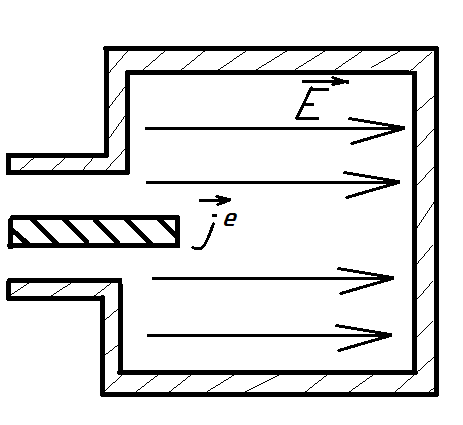
\includegraphics[width=0.25\linewidth]{aed_imgs/ask15_1} &
			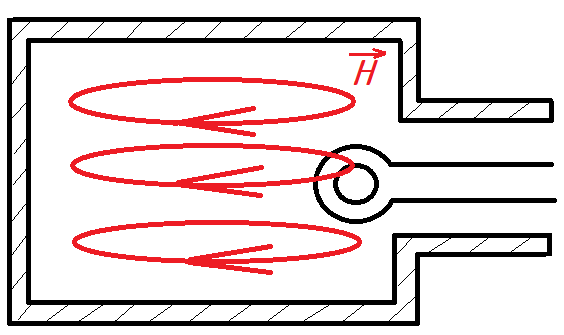
\includegraphics[width=0.25\linewidth]{aed_imgs/ask15_2} \\
			{штырь $\sim$ электрический диполь} & {петля $\sim$ магнитный диполь} \\
			\multicolumn{2}{c}{$\vec{P}\sim e^{i\w t}$} \\
			\multicolumn{2}{c}{Условия возбуждения:} \\
			{$\vec{J^e} \parallel\vec{P^e}$} & {$\vec{J^m} \parallel\vec{P^m}$} \\
			{$\vec{E_\text{р}} \parallel\vec{P^e}$} & {$\vec{H_\text{р}}\parallel\vec{P^m}$} \\
			\multicolumn{2}{c}{расположены в максимальном собственном поле резонатора} \\
		\end{tabular}\\
		Возбуждение штырём: в волноводе/резонаторе проделывается отверстие и вставляется штырь. Надо, чтобы вектор излучения электрического диполя был параллелен вектору напряженности электрического поля. Для максимального эффектра отверстие проделывается там, где электрическое поле наибольшее.\\
		Возбуждение петлёй: в волновод/резонатор вводится провод, загнутый крючком, и замыкается на стенке. Плоскость петли перпендикулярна линиям напряженности магнитного поля, т.е. направление вектора излучения магнитоного диполя сонаправлено с линиями напряженности магнитного поля.
		
		\section{Определения дифференциального и полного сечений рассеяния тела. Выражение для амплитуды поля и плотности потока энергии рассеянной волны в дальней зоне через дифференциальное сечение рассеяния.}
		
		Дифференциальное сечение рассеяния — отношение потока энергии излучения, рассеянного в единицу телесного угла к интенсивности падающего излучения (плотность полного сечения рассеяния по телесному углу)\\		
		$\sigma_\text{диф} = \dfrac{dP}{d\Omega S_\text{пад}}$, где $S_\text{пад}$ - величина вектора Пойтнинга в падающей волне\\
		$\Omega$ — телесный угол, $d\Omega = \dfrac{dS}{r^2}$\\
		$dP = |S_\text{расс}|dS$ - поток энергии, рассеиваемый телом в единицу телесного угла (мощность излучения в элемент телесного угла).\quad $dP = |S_\text{пад}|dS = 0$\\
		Полное сечение рассеяния - отношение полного потока энергии рассеянного излучения к интенсивности падающего излучения\\
		$\sigma_\text{полн} = \dfrac{{\text{П}_\text{расс}}}{S_\text{пад}} = \dfrac{\int_{4\pi}\sigma_\text{диф}\,d\Omega}{S_\text{пад}}$\\
		Определение дальней зоны: 1. $R \gg \lambda$;\quad 2. $R \gg l$;\quad 3. $\dfrac{\sqrt{\lambda R}}{l} \gg 1$\\
		$S_\text{расс} = \qty(\dfrac{\sigma_\text{диф}}{r^2})S_\text{пад}$ - плотность потока энергии\\
		$E_\text{расс} = E_\text{пад}\dfrac{\sqrt{\sigma_\text{диф}}}{r}$ - выражение для амплитуды поля\\
		
		\section{Приближение геометрической оптики и условия его применимости в задачах дифракции плоской волны на теле. Понятие луча и лучевой трубки.}
	
		1. $\lambda \ll L$, $L$ - характерный размер тела\\
		2. Падает плоский бесконечный пучок света\\
		3. Неприменим для острой границы и вблизи границы свет-тень\\
		4. При образовании каустик (поверхностей, где отражается бесконечное число лучей) $\vec{E} = \infty$\\
		5. Неприменим для фокуса линзы (или рядом с ним)\\
		Луч - линия, вдоль которой течет энергия. Лучи в лучевой трубке при отражении от выпуклой поверхности - расходятся, при отражении от вогнутой поверхности - сходятся.
		
	\end{multicols*}
\end{document}